\documentclass{beamer}


% Paquetes
\usepackage[T1]{fontenc}    % Para escribir en español
\usepackage{hyperref}    % Para hacer links a la web
\usepackage{listings}    % Para incluir código
\usepackage{graphicx}    % Para incluir imágenes

% Setup imagenes
\graphicspath{ {out/}}


% Estilos
\usetheme{Luebeck}


% Info para la title page
\title{Concurrencia a Museos de Argentina}
\subtitle{Relación con otros consumos culturales}
\author{Nazareno Magallanes \and Javier Spina \and Lautaro Terreno}
\institute[ECyT]
{
  Escuela de Ciencia y Tecnología
  \and
  Universidad Nacional de San Martín
}
\date{Noviembre 2022}


% Inicio del documento
\begin{document}

\frame{\titlepage}

\begin{frame}
\frametitle{Presentación del \textit{dataset}}

\begin{itemize}
\item<1-> Se trabajó con el \textit{dataset} asociado a la \textbf{Encuesta Nacional de Consumos Culturales} realizada en 2017. Son datos abiertos del Ministerio de Cultura de la Nación, disponible en \href{https://datos.cultura.gob.ar/dataset/encuesta-nacional-de-consumos-culturales-2017}{su página web.}
\item<2-> Además del archivo \textit{csv}, se contó con el cuestionario aplicado y el Informe General realizado por el mismo Ministerio.
\item<3->El \textit{dataset} consta de 2802 unidades de análisis y 450 variables. Cada una de las variables se corresponde con las preguntas del cuestionario asociado.
\item <4->Cada unidad de análisis es una persona encuestada.
\end{itemize}

\end{frame}

\begin{frame}[fragile]
\frametitle{Un primer vistazo}

\begin{itemize}
\item<1->Para comenzar a trabajar con el \textit{dataset} se debió resolver fundamentalmente la cuestión de los nombres de las variables: 

\begin{lstlisting}
> colnames(encuesta)
[1] "id"  "pondera_dem"  "fecha"  "region"
[5] "sexo"  "edad"  "p1"  "p1otros"
[9] "p2"  "p2_1"  "p2_1otro"  "p2_2"
[13] "p3"  "p4"  "p5"  "p6horas"
\end{lstlisting}

\item<2->La gran mayoría de las variables es de la forma: p + <número de pregunta del cuestionario>.
\end{itemize}

\end{frame}

\begin{frame}
\frametitle{Limpieza de datos}

\begin{itemize}
\item<1-> Se transformaron los nombres de las variables considerando la pregunta asociada del cuestionario. Por ejemplo, p98 se renombró a concurre\_museo porque se corresponde a la pregunta 98: ¿Concurrió a algún museo durante el último año?
\item<2-> Se debieron eliminar 2 unidades de análisis que estaban mal cargadas.
\end{itemize}

\end{frame}

\begin{frame}
\frametitle{Búsqueda de la problemática}

Luego de varias iteraciones de lectura y interpretación de los datos, diversas pruebas y errores, se vió que el Informe General señalaba una problematica: hay una tendencia negativa en la concurrencia a los museos argentinos en determinados sectores sociales.

\begin{block}{La pregunta}
¿Cómo aumentar la concurrencia a los museos?
\end{block}

\end{frame}

\begin{frame}
\frametitle{La pregunta y su contexto}

\begin{block}{Contexto}
\begin{figure}
\centering
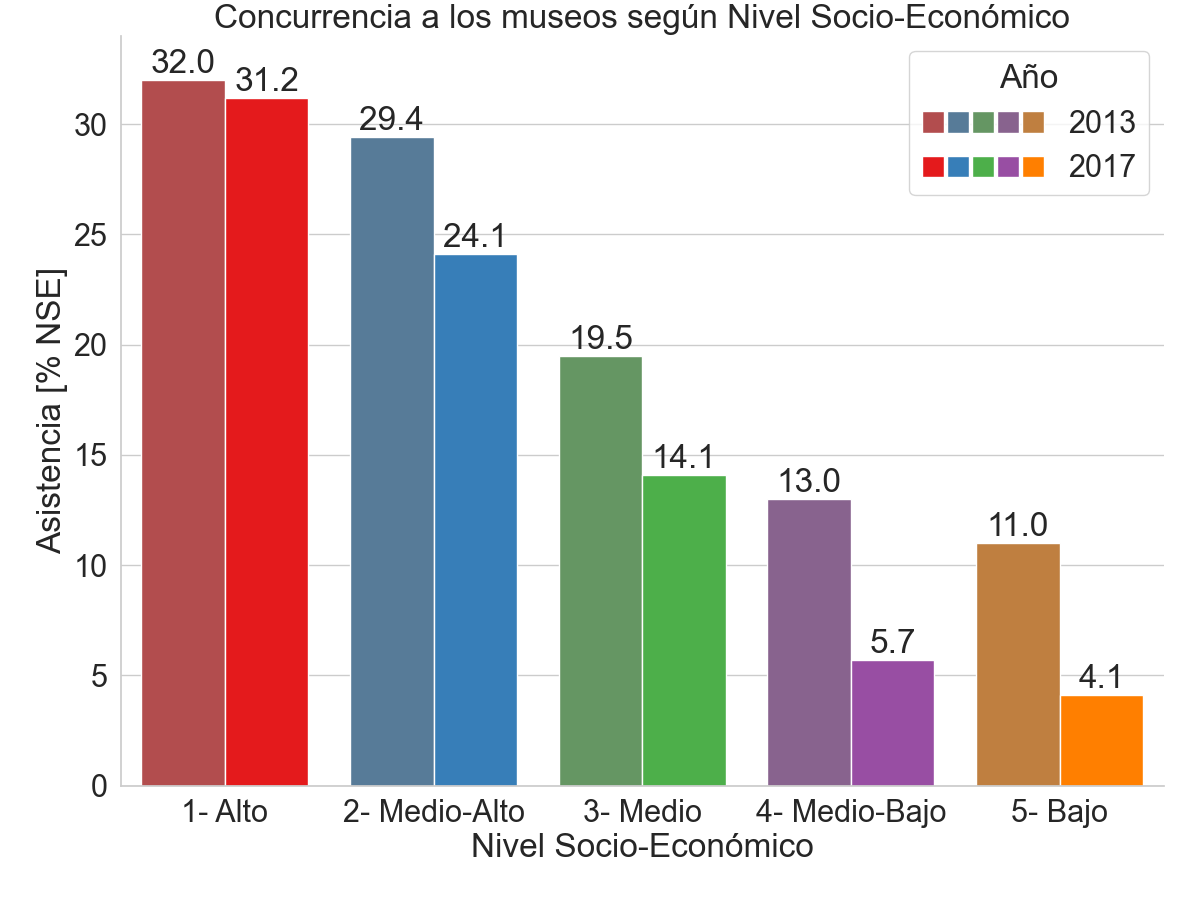
\includegraphics[height=0.6\textheight]{asist_museo_nse_x100}
\label{fig:asist_museo_nse}
\end{figure}


%Poner acá primeros gráficos parecidos a los de la página 23 del informe para mostrar contexto. Quizá alguno más puede aportar, hay que ver cuál.
%Quizá apoyarnos con el dataset extra de ubicaciones de los museos en el país, considerar si el factor de que la gente no tiene ni 1 auto en el nivel socio económico q no está yendo a museo.

\end{block}

\end{frame}

\begin{frame}
\frametitle{Estrategia para responder la pregunta}

Acá hablar de que buscamos de los que SI fueron a museo tuvieron ciertos preferencias en otros consumos culturales como música, tv, películas. 
Teniendo en cuenta esa segmentación, buscar a la gente que tiene esas preferencias y NO fue a museos y proponer esto como estrategia para alentar la concurrencia, invocando el dato de q 75 por ciento  de la gente que fue a museo no pagó entrada. 
Osea sugerir una semana de los museos como la noche de los museos con entrada gratis para q la gente pueda ir.

Se pueden meter los modelos acá también, poner en Eje X la edad, en Eje Y NSEpuntaje (más bajo, menor clase social, más álto el puntaje mayor clase social) y buscar modelar ahí y ajustar por cantidad de autos, si concurrió o no a museo, por región, etc. No estoy seguro q sale de eso.

\end{frame}

\end{document}
